%!TEX root = ../thesis.tex
%*******************************************************************************
%****************************** Fourth Chapter *********************************
%*******************************************************************************

\chapter{Design of impedance plethysmography device}
\label{chapter design}

\ifpdf
    \graphicspath{{Chapter4/Figs/Raster/}{Chapter4/Figs/PDF/}{Chapter4/Figs/}}
\else
    \graphicspath{{Chapter4/Figs/Vector/}{Chapter4/Figs/}}
\fi


%********************************** %First Section  **************************************
It is well known that detecting changes in volume in the human body, provides valuable medical information. Ischemia is known as lack of blood supply towards an organ or tissue. Most common cases occur when there is a blockage in an artery. Thus, leading to tissue starvation because of lack of oxygen and nutrients. One of the most common diseases that involves extremities is the peripheral arterial disease. This disease is a progressive vascular illness caused by blockage, narrowing or spasms in blood vessels such as arteries, veins or lymphatic vessels. Referring to limbs, these represent a significant cause of disability and mortality~\cite{novo1995patients}. Knowing patient's haemodynamic conditions may help medical therapists to follow an appropriate plan of treatment according to the severity of the condition.

Electrical impedance plethysmography is a method non-invasive, portable, comfortable, safe, unperceivable, straightforward and easy to implement.  It can detect changes in blood volume not just in the periphery but also other parts of the body. In short, this method takes advantage of blood and tissue conductive properties. It has a resistive response when an alternating current is applied. Ionic conduction of a segment of the body reflects the same behaviour of electric conduction in metallic cylinders. Since 1950's, it has been extensively proved that changes in arteriovenous blood volume in an extremity segment is directly related to static and dynamic changes of impedance measurements in synchrony with the heart cycle.

The genesis of impedance plethysmography can be traced back to the model proposed by Jan Nyober~\cite{nyober1950electrical}. The author describes extremities as cylinders. The whole electrical conductance path is resulting from the sum of the parallel conductance of blood and tissue within a segment. In fact, this theory called parallel conductor was later confirmed by the experiments performed by Shimazu et al~\cite{shimazu1982evaluation}. There have been some doubts about how much is blood's impedance contribution to the total impedance signal.  It has been demonstrated through in vitro experiments that blood (haematocrit = $ 26 \pm 4 \%$) contributed to \SI{10}{\percent} of the signal. In the test, a saline buffer solution was compared between extensible arteries and rigid tubes~\cite{peura1978influence}. 

Nyober proposed that the practical parallel resistive value of the displaced blood can be originated from the parallel relation between the initial base resistance and the new resistance value, given by the following expression:

\begin{align}
R_B=\frac{R_N R_0}{R_0-R_N} \approx \frac{R^2_0}{\Delta R}
\end{align}

where $R_0$ is equivalent to the original resistance and $R_N$ represents the increase of new total resistance. The denominator $R_0 - R_N$ is equal to $R$, peers with the change of impedance caused by blood volume expansion during the heart cycle. From this, the author deducted the following governing equation. That shows that proportional increment of blood volume uniformly distributed within a cylindrical segment can be derived from the equation of the volume of a cylindrical conductor:

\begin{align}
 \label{eq:Nyober}
 V_B = \rho \frac{l^2}{R_B}
\end{align}

where $\rho$ is blood's resistivity, $l$ is the distance between measuring electrodes, and $R_B$ is the impedance value described previously as the parallel value of resistances.

Different equations aroused complementing the Nyboer's work. One of this modifications is the Kubicek et al. method~\cite{karnegis1966development}. His equation is widely used especially when measurements from the measurement of impedance cardiography from the thoracic box and to deduct stroke volume of the heart. Other, popular work is the contribution done by Sramek~\cite{sramek1986bomed}. The author also modified Kubicek's equation eliminating the dependence $l$ and $\rho$,  and introduced a constant obtained from statistical methods named "volume of electrical participating tissue". 

\mynote{This is not clear, needs to be refined}

From the equations named previously, it is possible to obtain a different kind of haemodynamic information. The most common used as describe before is plethysmography information based on the principle described. However, various applications have been applied to the signals obtained from impedance plethysmography. 

For instance, some measurements require changes in the basal impedance which is the base impedance for tissue, fat, skin, bone and blood when there is no expansion of volume. For better understanding this can be described as the DC content of a signal or in the case of Nyober's parallel conductor is equivalent to $R_B$. This impedance value is particularly attractive when estimating blood flow in extremities. The method that uses this kind of data is referred as venous occlusion plethysmography. In this approach, a cuff is inflated \SIrange{10}{20}{\mmHg} below systolic for a period and then released. Some of its applications can be seen being applied in the study performed by Mohapatra~\cite{mohapatra1979measurement} and Schraibman~\cite{schraibman1975comparison}, where a comparison of the change of volume using strain gauge and impedance in patients under anaesthesia showed a significant relationship between both techniques.{eq:nyober}

Yamakoshi~\cite{shimazu1982evaluation,yamakoshi1980limb,yamakoshi1978admittance}  in his research and patent work also uses the same method to estimate blood flow but instead of using impedance uses its reciprocate admittance $(Y=Z^{-1})$ for natural computational results. In his work, the author states that the first gradient of the computation result to time is indicative of the blood rate in the limb being examined.
 
The plethysmography waveform is also utilised to quantify measurements of pulsatile volume, blood flow beat to beat, blood pressure and pulse wave velocity. In this case, the waveform is equivalent to the AC component of the impedance signal. The contribution of this signal to the total of the signal is between \SIrange{0.1}{1}{\percent} of the total of the signal. Sometimes, it is necessary to implement low noise techniques to picking up the signal hidden within the basal impedance. 

The most typical application of the waveform is the quantification of blood flow beat to beat. Compared with the previous technique, this method does not require venous occlusion. By applying Nyboer's equation to the waveform signal is also possible to quantify peak-peak blood volume and peak net inflow. For instance, the patent presented by Marks~\cite{marks1985computer} shows the application of quantifying blood flow in upper extremities by computing the derivatives of the waveform signal producing the results claimed. Another example, taking measurements from lower limbs is the work performed by Porter~\cite{porter1985measurement} where impedance cardiography was used to obtain the waveform signals and computed using Kubicek's equation and concluding the potential use of the signal to evaluate limb oedema. 
{eq:dvdr}
Another application of the waveform is the evaluation of blood pressure continuously. Blinov~\cite{blinov1997plethysmographic} demonstrated that pressure could be deducted if blood flow is known. As explained before, blood flow can be estimated beat-beat by deriving the waveform after applying Nyober's equation. As a result, the equation transforms into:

\begin{align}
\label{eq:dvdr}
dV = \rho \frac{l^2}{R^2_B} dR
\end{align}

Volume rate is defined as the change of volume in time. Then blood flow rate $(\dot{Q})$ is defined by the following equation:

\begin{align}
\dot{Q} = \frac{dV}{dt}=-\rho \frac{l^2}{R^{2}_{B}} \frac{dR}{dt}
\end{align}

where $W$ is the hydraulic resistance and $P$ is pressure. The hydraulic resistance is a function of the geometry of the artery given by radius $r$ and the viscosity of the blood $\mu$.

\begin{align}
W=\frac{8 l \mu}{\pi r^4}
\end{align}

Replacing equation $W$ into equation $\dot{Q}$ the pressure for a defined segment can be expressed by the following equation:

\begin{align}
P = -\frac{8 l \mu \pi}{\rho} \frac{dR}{dt} = k \frac{dR}{dt}
\end{align}

where $k$ is a constant value function of the distance between the electrodes, physiological constants of the blood at a particular measurement frequency. The sign in the equation just denotes that the changes in the resistance and pressure are opposite. Thus the sign can be disregarded while performing calculations.

Finally, the waveform obtained from impedance plethysmography can also be applied to evaluate pulse-wave velocity (PWV) in limbs. Measuring PWV can be accomplished by computing the time arrival difference between two reference measurement points and estimating the time difference between both waveforms. PWV is also an important indicator of deterioration in the cardiovascular system. This method requires two or more electrode arrays to measure the differential of electrical potential along a body segment. For its convince is easily applied to upper and lower limbs. This measurement technology has been successfully demonstrated by some researchers like Risacher et al~\cite{risacher1993impedance} where measurements were recorded using a multi-array electrode system. Some of the recommendations to the successful application of this method recommended by the author are taken special emphasis in the sensitivity to noise that this method may come across~\cite{risacher1992computation}, the use of high-precision and reproducible by the electrode array, accuracy in the measurement of the distance separating measuring sites, high sampling frequency to ensure higher accuracy in the calculation of time intervals. There are limits when recording these signals from a small body where location and geometry of the electrodes are prime for this application. It has been shown that is possible to record this signal from an area as small as \SI{1.5}{\cm} by \SI{7}{\cm} which also increases the possibility of portability~\cite{cho2009bio}. 

As it can be noticed, there are multiple applications where impedance plethysmography can be applied, but so far this has been achieved by devices that can only provide only either basal impedance (DC), waveform (AC) and single channel application. The aim of this work is to design a device that can be used for any to study any of the previous applications using a single apparatus. This device should be able to provide the characteristics described in a multi-channel device.  

\section{Material and methods}
Designing an impedance device requires knowing the electrical characteristics of the load under test. Nonetheless, some of the recommendations should start with meeting patient's safety. Meaning, that the amount of current to be driven by the device should be imperceptible within the limits of the safety standards. For this, one of the first recommendation is to be able to operate by batteries as a class B device, ensuring that electrical currents are floating in the patient and also guarantying that current will be flowing through the segment to be studied. Levels of current sensation change from person–to–person, sex and also depends on the electrode's geometry. However, Brown et al.~\cite{brown1998medical} has established a threshold current which is frequency dependent where \SI{5}{\mA} represent the limit for sensory nerve stimulation and shock sensation. The device designed can deliver four levels of current using a dip-switch (\SIlist{1;2;3;4}{\mA}). For the experiment of this document, the current was fixed to \SI{4}{\mA} which provided and an excellent sensitivity for the system. 

About the electrical current delivered by the device, a programmable wave generator with the potential of delivering up to 10 MHz sinusoidal waveforms was incorporated into the design. However, as per the literature measuring impedance plethysmography can be achieved with frequencies between \SIrange[scientific-notation = engineering]{20}{200000}{\hertz}. Therefore, a sinusoidal wave of \SI{50}{\kilo\hertz} was used during the experimental procedure.

\subsection{Electrodes topology and location}
There are two kinds of impedance plethysmography method according to the electrode topology, bipolar and tetrapolar. Bipolar lacks two electrodes points to measure impedance. When measuring with bipolar electrodes arises a problem where the impedance of the electrodes might be greater than the biological tissue itself which can affect the measurement significantly. In the majority of the cases, it is quite difficult to differentiate the electrode's impedance from the tissue one \cite{brown2000bipolar}. Tetrapolar configuration requires four contact points, a pair of electrodes injects current and another couple sense voltage. Using tetrapolar arrangement minimises the voltage drop during measurements because the potential sensing amplifier ideally has a bigger impedance compared to the interface electrode-skin. Therefore, electrical current would not flow between electrodes and the voltage amplifier. For this reason, four electrodes measurement was decided as the optimal method while designing the instrument. 

Positioning the electrodes close to the main vessel improves the response of the system as the there is more conductive material where the electrical current can flow through. Figure~\ref{fig:electrode} shows in more detail the position of the electrodes to take measurements from the device. According to the arm anatomy, the radial artery is the proper site to use for one of the current electrodes. The other was placed close to the brachial artery around the cubital fossa region where this vessel is closer to the surface. The sensing electrodes were placed right on the elbow where is the nearest point to the brachial artery that is connected to the radial artery forming the ideal loop to detect changes in impedance $\Delta Z$.  

\begin{figure}[!htpb]
	\centering
	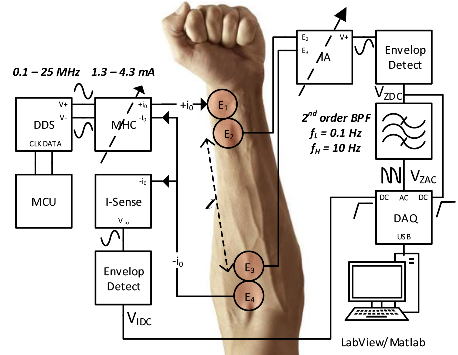
\includegraphics[width=7.75cm,keepaspectratio]{figure1}	
    \caption{Electrode placement in forearm}
    \label{fig:electrode}
\end{figure}

The proposed system can be subdivided into two different sections, front–end which is the part of the device that interacts directly with the limb under test and the back–end that performs the wave generation, signal conditioning, computational calculation, and data representation. The following image shows the block diagram of the proposed device.

\begin{figure}[!htpb]
	\centering
	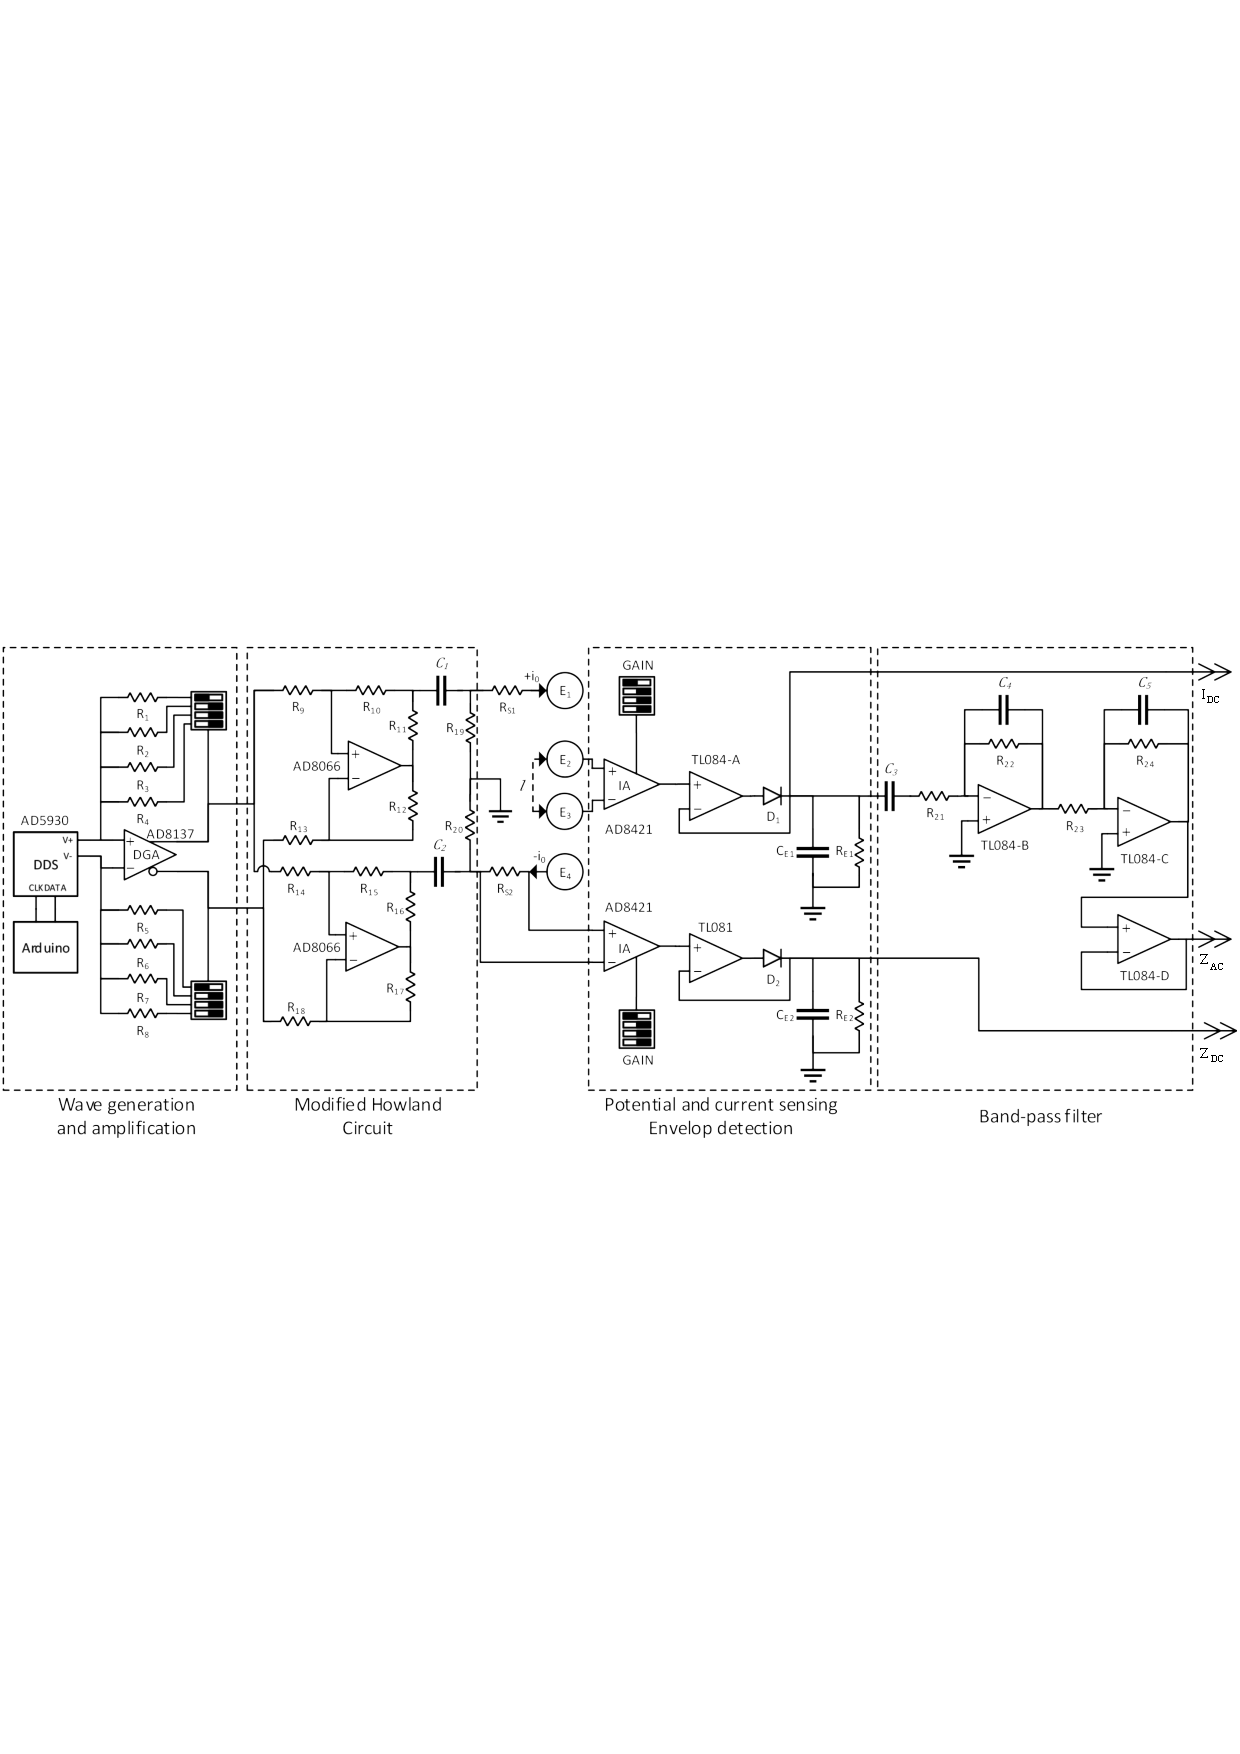
\includegraphics[width=\textwidth,keepaspectratio]{figure2}
    \caption{Block diagram of impedance plethysmography device}
    \label{fig:block}
\end{figure}

\mynote{I need to add ports names of the device}

\subsection{Power supply}
Implementing a good design requires good power supplies that could provide steady voltage output and supply enough current as needed by the circuitry. Due to the need of applying floating currents, a power supply was designed to operate with batteries minimising ground loops and increasing patient's safety.  The selection of this method of supplying power lessens the likelihood of electric shocks as well as reaching dangerous voltage levels. For these reasons, a couple of batteries A512/2 S (Sonnenschein) were used to power all the circuits. These cells provide \SI{2}{\ampere\hour} of capacity per bank.

Some of the unique features needed for the power supply includes the capability of providing a dual voltage (\SI{\pm 12}{\volt}) as some Op–Amps require this level of supply to achieve maximum gain and low energy supply (\SI{5}{\volt}) essential for some digital components. The positive and negative voltages can be obtained by using one cell bank with normal polarisation and the other inverted. 

In summary, the following table describes the characteristics and IC's used in the power supply module. Including level voltages, output current per channel and the specific function of each voltage level. 

\begin{table}[!htpb]
	\caption{Components of the Power Supply and its functions}
	\centering
	\label{table:power supply details}
	\begin{tabular}{p{2 cm} p{2 cm} c p{6 cm}}
		\toprule
		\textbf{Voltage supply} & \textbf{Current supply} & \textbf{IC} & \textbf{Function} \\ 
		\midrule
		+\SI{12}{\volt} & \SI{1.5}{\ampere} & LM317 & Power supply for single and dual Op-Amps, In-Amps and as power supply for +\SI{5}{\volt} \\ 
		\midrule 
		-\SI{12}{\volt} & \SI{1.5}{\ampere} & LM337 & Negative power supply for single and dual Op-Amps and In-Amps \\ 
		\midrule 
		\SI{5}{\volt} & \SI{100}{\milli\ampere} & AP117E50G & Power supply for digital components working at TTL level \\ 
		\bottomrule 
	\end{tabular}
\end{table}

The schematic circuits for the power supply designed are shown in the appendix \ref{Appendix: Power Supply}, figure \ref{Appendix: Power Supply}. To operate the iPG device requires positive (VIN+) and negative (VIN–) supplies that can be provided by any external power, for safety batteries was the source of choice. The table \ref{table:power supply details} shows the components employed in the implementation, which operates within the desired appropriate range required by the device. The regulators LM3XX are voltage variable regulators. However, their output was set to \SI{\pm 12}{\volt} for each source, using the appropriate selection of resistors. The capacitors added to each of the regulators were selected according to the manufacturer’s recommendation to avoid any ripple at the output voltage.

\begin{figure}[!htpb]
	\centering
	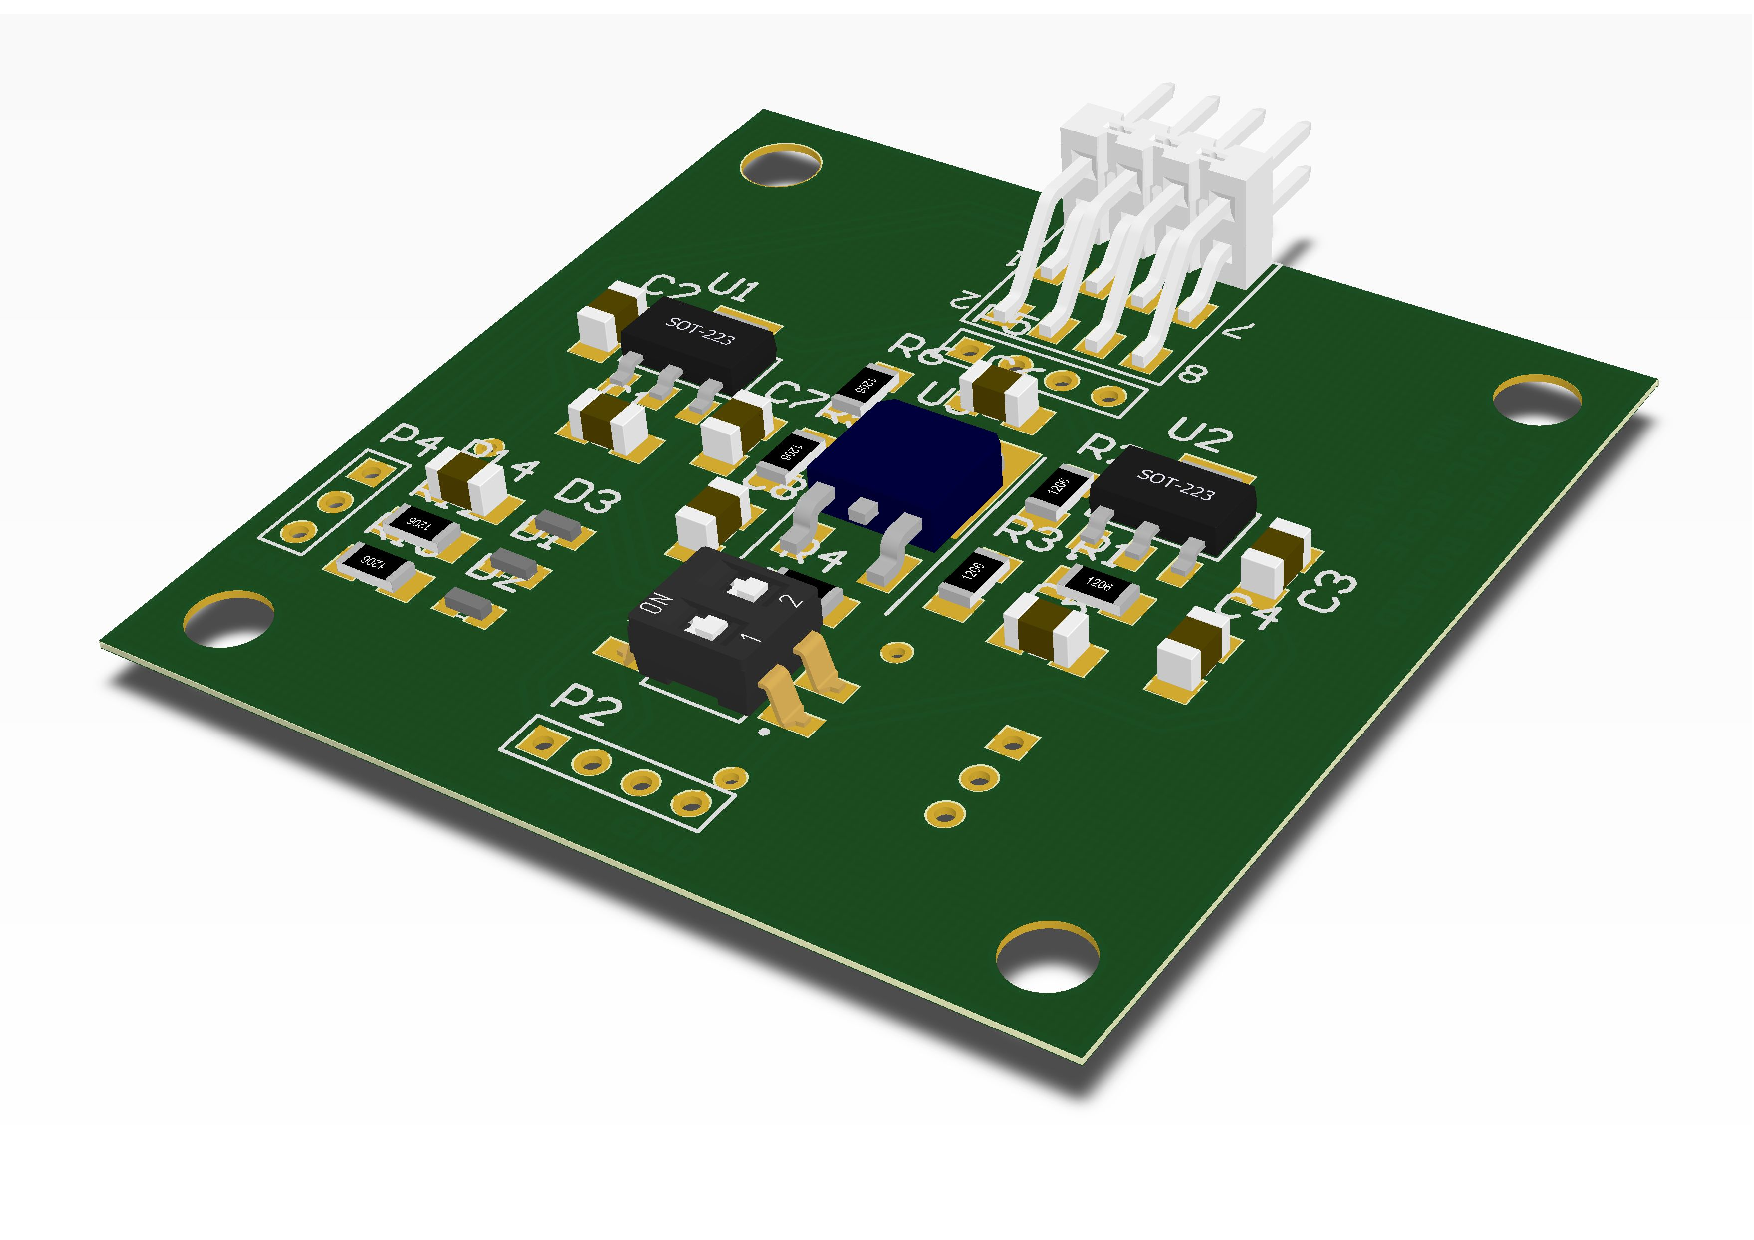
\includegraphics[width=7.5 cm,keepaspectratio]{figure_PS}
	\caption{3D View of the Power Supply designed}
	\label{fig:3D PS}
\end{figure}

In Altium Designer a PCB of \SI{50}{\milli\meter} x \SI{50}{\milli\meter} was produced considering input and ports as well as indicators and sensors. For instance, the ports included three input voltage pins VIN+, VIN– and ground (GND) coming from the batteries, an eight-pin male connector that provides regulated board to the next board. The indicators and sensors included a dip-switch working as power ON/OFF button, a set of three red-LED indicating the power of +\SI{12}{\volt}, -\SI{12}{\volt} and \SI{5}{\volt}, a three-pin port that connects to the ADC port of the microcontroller which monitors the batteries capacity. It also includes additional regulated voltage ports to feed other external modules.

The final result can be appreciated in \ref{fig:3D PS}, where the 3D model representation from Altium design and the final PCB manufactured using LPKF machine are displayed side by side. \mynote{Check if I want to add the real picture}


\subsection{Direct digital synthesis (DDS)}
Following the block diagram from left to right on figure \ref{fig:block}, the first part shows the wave generator. This section of the circuit produces the sinusoidal wave needed for the impedance measurements. This waveform should be low in distortion and noise. This signal was created using a programmable direct digital synthesis (DDS) integrated circuit (IC) which is capable of producing sine waves from \SI{10}{\hertz} to \SI{10}{\mega\hertz}. The IC used is the AD5930 (Analogue devices). In short, a DDS creates a wave according to a table of digital words in memory which are fed to a DAC that produces the analogue equivalent. This IC requires a set of instruction to operate. 

In the appendix \ref{Appendix: DDS PS}, the figure \ref{fig:DDS PS} shows the schematic used in the design of the wave generator. Due to the noise that a digital circuit would feed into an analogue system, a separate power supply powers up this module. For this two voltage regulators (AP117E50G) provide \SI{5}{\volt} sources of energy for digital and analogue components, using two separated ground paths (GND - AGND). Also, a \SI{3}{\volt} reference is needed for the oscillator to operate which is supplied by the IC REF196. The DDS requires an external clock to work. Therefore a \SI{50}{\mega\hertz} oscillator provides the clock signal needed.

\begin{figure}[!htpb]
	\centering
	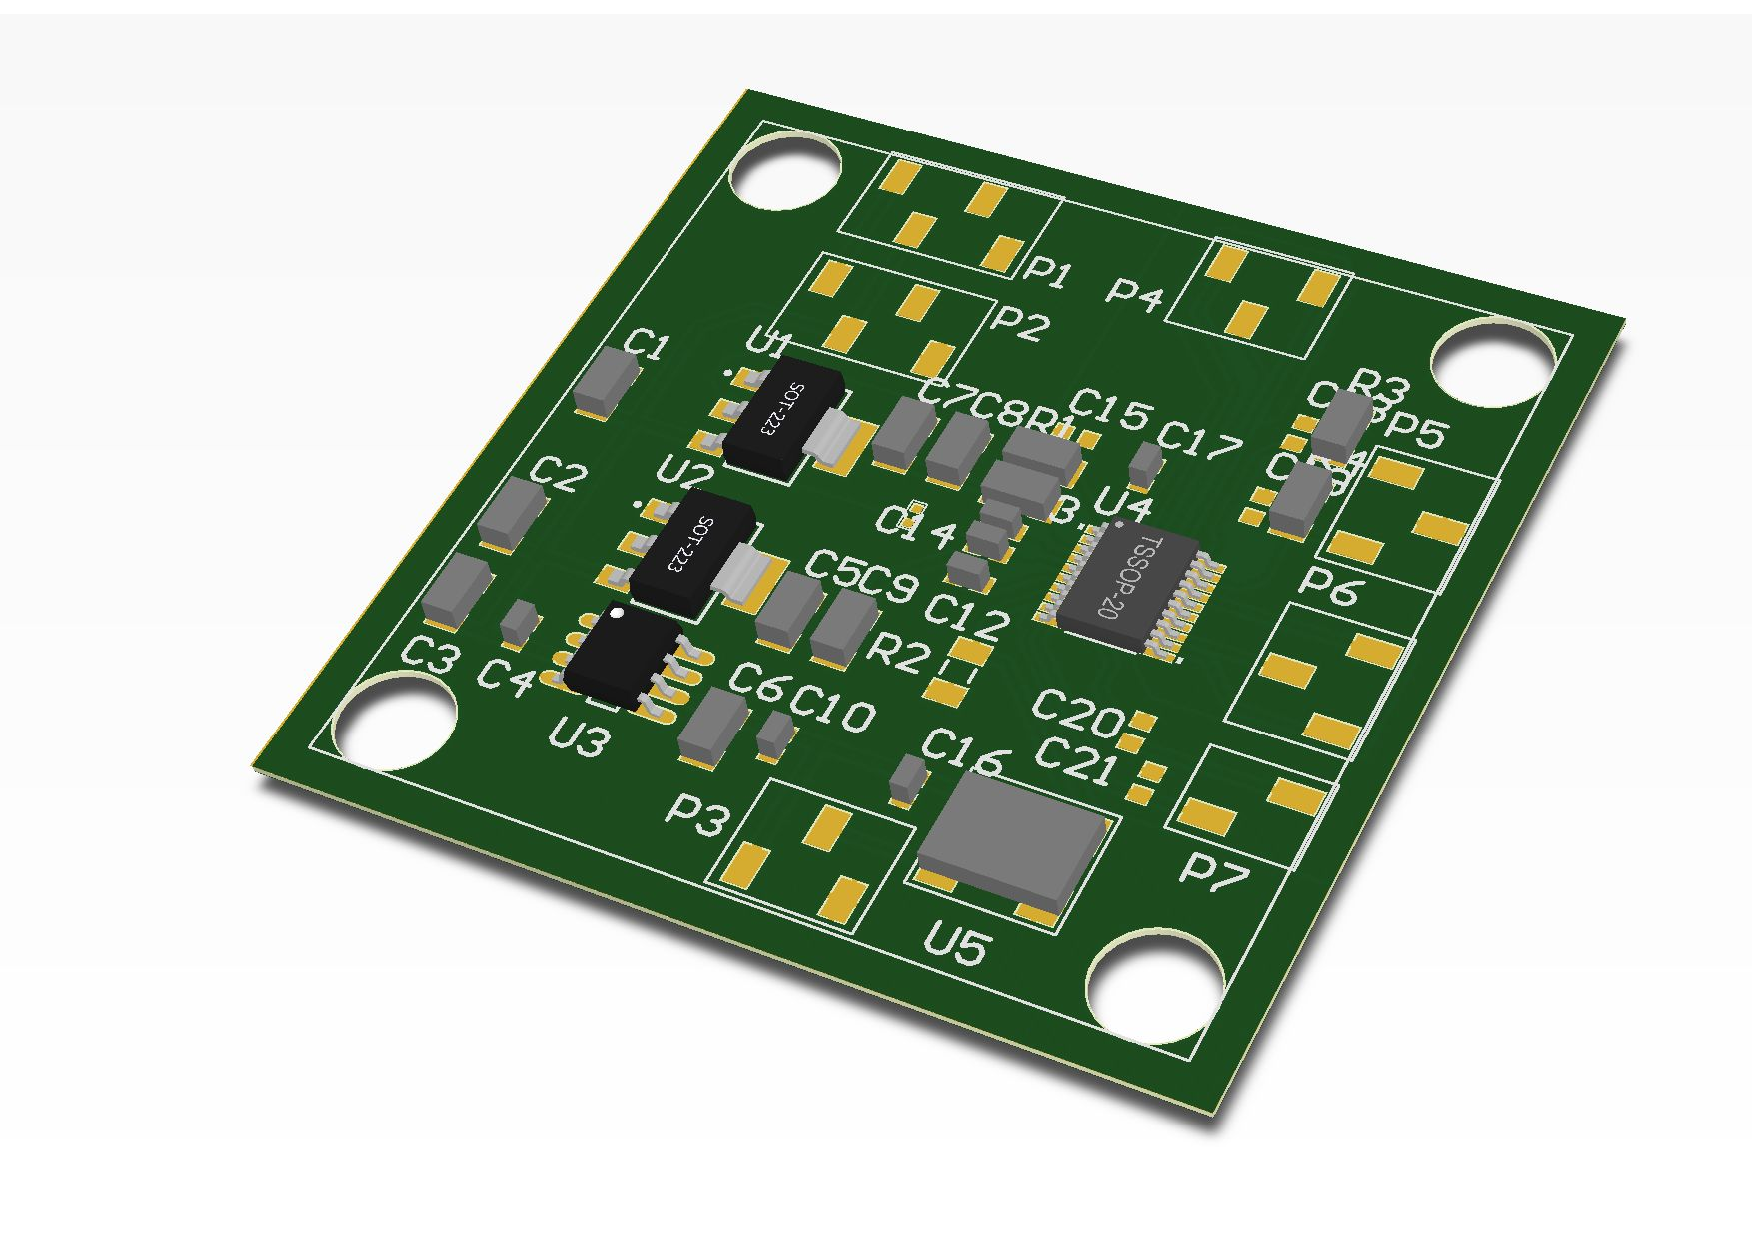
\includegraphics[width=7.5 cm,keepaspectratio]{figure_DDS}
	\caption{3D representation of the DDS module PCB}
	\label{fig:3D DDS}
\end{figure}

A microcontroller ATMEL (Arduino) controls the DDS sending commands via serial peripheral interface bus (SPI) transmission interface. Through an instruction set by the manufacturer, it is possible to set the oscillation frequency of the sine wave, as well as start/stop the signal generation. The waveform generated by the DDS is differential, meaning that there are two sine waves outputs in counter-phase (\SIlist{0;180}{\degree}). The DDS provides a current output of \SI{3}{\mA} which is transformed to an electrical voltage using a \SI{200}{\ohm} resistor at the output of the IC, setting the output at approximately \SI{600}{\mV}. A set of capacitors also filters high-frequency noises. The connection between the microcontroller and other boards is possible using ribbon cables. The figure \ref{fig:3D DDS} shows the 3D representation of PCB module manufactured.

\subsection{Differential amplifier gain}
The following stage consists of a differential voltage amplifier. The gain of this amplifier can be modified by using a set of resistors at each side of the amplifier and can be set to 16 different combinations of gain using resistors of \SIlist{2;3;5;6}{\kohm}. As a result, DDS’ output voltage changes according to gain set in the differential amplifier. 

\subsection{Modified Howland Amplifier}


Then a transconductance amplifier is used to convert the voltage coming out from the differential amplifier into an electrical current. By driving current instead of voltage, a greater control is achieved because only the current selected will be passing through the patient. The configuration chosen is a modified Howland circuit set to \SI{1}{\milli\siemens} of gain.
 
The Op–Amp selected for this design was the AD8066 (Analog Devices); which is a dual Op–Amp that offers high bandwidth of \SI{145}{\mega\hertz}, high input impedance of \SI{1000}{\giga\ohm} @ \SI{4.5}{\pF}, low noise of \SI{7}{\nano\volt\per\sqrt{Hz}} at \SI{10}{\kilo\hertz}, open loop gain of \SI{113}{\decibel} and CMMR of -\SI{100}{\decibel}~\cite{ad:AD8066}. All these characteristics made this Op–Amp ideal choice implementing MHC.

\mynote{Add graphics according to the description on each file}

\begin{figure}[!htpb]
	\centering
	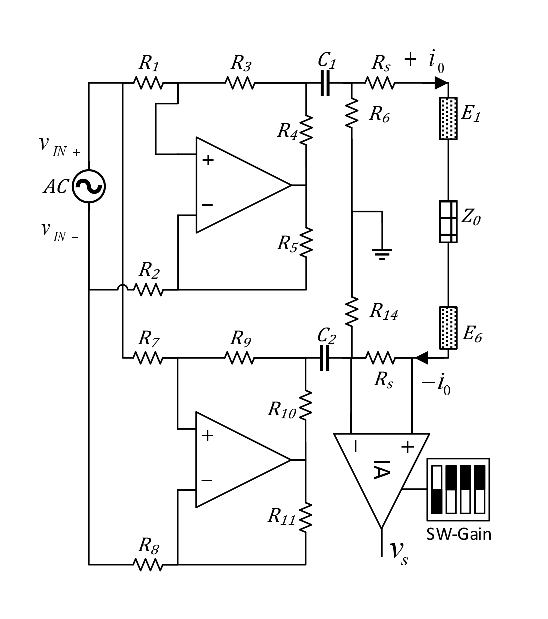
\includegraphics[width=9cm,keepaspectratio]{figure3}  
    \caption{Modified Howland circuit schematic}
    \label{fig:mhc}
\end{figure}

The MHC design requires low tolerance resistors to minimize potential errors introduced to the system. Consequently, resistors of \SIlist{1;100}{\kohm} with a tolerance of \SI{0.1}{\percent} were used in the final implementation. Figure \ref{fig:mhc} shows the schematic implemented of the differential MHC, only the top Op–Amp is analysed to prove that the equivalence was met, the one on the bottom follows the same equations but with inverted output. The circuit’s resistors from the equation are equivalent to the followings: $R_{2A}=R_1, R_{2B}=R_2, R_1 = R_3 + R_4, R_3 = R_5$ and $R_4 = R_6$. Thus, the equivalent equation can be re-written as follows: 

\begin{align}
\label{eq:Req}
\frac{R_1 + R_2}{R_3 + R_4} = \frac{R_6}{R_5}
\end{align}

where $R_1=R_4=R_5=R_6=100K\Omega$ and $R_2=R_3=1K\Omega$. Finally, the resistor equivalence is calculated as shown by equation \ref{eq:Req}. 

The transconductance of this circuit was calculated from equations \ref{eq:Req}. Following the same resistors equivalence previously described, the positive  transconductance $(G^+_m)$ and negative transconductance $(G^-_m)$ were calculated as described by the following arithmetical operations:


\begin{align}
\label{eq:G+}
G^+_m=\frac{i_{out}}{v_{in+}}=\frac{100K\Omega + 1K\Omega}{101K\Omega \times 1K\Omega}=\frac{101K\Omega}{101M\Omega}=1\times10^{-3}S 
\end{align}

\begin{align}
\label{eq:G-}
G^-_m=-\frac{i_{out}}{v_{in-}}=\frac{100K\Omega + 1K\Omega}{101K\Omega \times 1K\Omega}=\frac{101K\Omega}{101M\Omega}=-1\times10^{-3}S 
\end{align}

As it can be seen from \ref{eq:G+} and \ref{eq:G-}, the transconductance in both feedbacks is equivalent to \SI{1}{\milli\siemens}. The negative sign in $G^{-}_m$ is caused by a phase shift of \SI{180}{\degree}. Due to both top and bottom Op–Amps showed in Figure 3 having the same design, the total transconductance of the circuit in differential mode is equal to \SI{1}{\milli\siemens}. In other words, per every volt generated at the input (pins input– and input+) the output produces \SI{1}{\mA} of electric current. By interfacing the previous with this one, it is possible to deliver four different levels of current \SIlist{1.33;2.16;3.60;4.36}{\mA}.

\subsection{Current Sensing Circuit}
As shown from figure 3, at the output of the transconductance amplifier there are \SI{10}{\ohm} resistors at each side of the differential output. These small resistors have been placed there to sense the current being driven into the patient. Using Ohm's law $v=R \times i$ is possible to convert the current passing through that line into voltage. However, because the flowing current is in the order of $mA$ and resistor value is quite small, the voltage obtained is in the order of $mV$. Consequently, the resultant voltage is too close to the noise level, distorting the real value and not being able to be correctly detected by any analogue to digital converter. This can be complemented by using a high input impedance amplifier avoiding any current leakage through the current sensing IC.  

The most suitable device for this design was the In–Amp AD8421~\cite{ad:AD8421}. Some of this device's features are the low noise of \SI{3.2}{\nano\volt\per\sqrt{Hz}} at \SI{1}{\kHz}, high bandwidth 10 MHz when gain is unitary, high CMRR of \SI{80}{\decibel} at \SI{20}{\kHz} and dual supply operation within the range of the power supply designed [19]. This component also includes adjustable gain using external resistors between pin 2 and 3. In fact, a four dip-switch was set with four different resistor values that allow changing the gain of the current detection. This ensures that if a low value of current (\SI{1.3}{\mA}) is used, it is possible to adjust the gain of this stage to obtain a more accurate reading. The signal obtained is later passed through a peak detector explain in the section envelope detection circuit, that produces the signal that is fed to the ADC to be quantified by the back-end software. 

\subsection{Voltage sensing circuit}
\label{section design 1.5}
A sensing circuit was created according to design theory explained in section. This circuit as its name implies senses or captures the output voltage coming from the unknown impedance in the limb segment. Likewise, the current injection design, this electric circuit requires high-quality components with high input impedance, high bandwidth over the frequency of interest, high CMRR and dual power supply capability compatible the power supply designed. Hence, the IC used in the previous section meet all the requirements. 

\begin{figure}[!htpb]
	\centering
	\dummyfig{Peak detection circuit} 
    \caption{Voltage sensing circuit schematic}
    \label{fig:sensing}
\end{figure}

The AD8421\cite{ad:AD8421} with its robust input impedance of and typical input bias current of \SI{1}{\nA} guarantees that the voltage drop from the interface electrode-skin is minimum. It can be calculated that the maximum error introduced by this voltage drop is close to \SI{0.0001}{\percent} per mA flowing through the body segment. 

The gain of the IC can be modified using its gain pins increasing the dynamic range of the sensing circuit. Consequently, a dip-switch 4 SPST was used to provide 16 different combinations of amplification which can be adapted according to the nature of the signal. Each channel has different gain combinations as shown in the following tables.

\begin{table}
    \label{tbl:rch1}
    \caption{Resistor configuration for Channel 1}
    \dummyfig{Block diagram} 
\end{table} 

\begin{table}
    \label{tbl:rch2}
    \caption{Resistor configuration for Channel 2}
    \dummyfig{Block diagram} 
\end{table} 


\subsection{Envelope detection circuit}
This circuit produces a DC voltage equivalent to the limb's impedance and extracts the pulsating signal (AC) from the impedance signal (DC). An active diode configuration derives the AC waveform. This circuit was created with an Op-Amp TL08XX\cite{ti:TL08xx} and a diode 1N4148. The combination of these two components create a ''super diode'' or ''perfect diode''. Indeed, the Op-Amp complements voltage loses of the diode where the voltage drop of the diode is compensated. The negative feedback created from the output of the diode towards the negative pin of the Op-Amp compensates diode's voltage drop. As a consequence, the input signal $Z_{in}$ coming into the signal is half-wave rectified crossing by zero. 

\begin{figure}[!htpb]
	\centering
	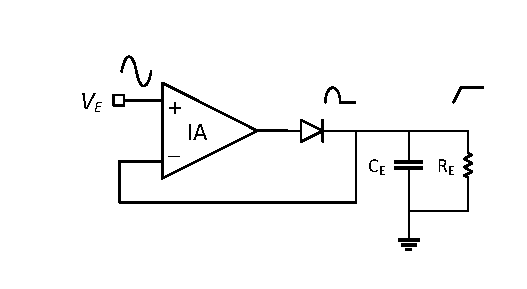
\includegraphics[width=7.3cm,keepaspectratio]{figure5}
 	\caption{Envelope detection circuit schematic}
    \label{fig:envelope}
\end{figure}

The signal obtained for the super diode circuit is passed to a hold circuit. The RC configuration keeps its charge until of the circuit, the selected by the impedance plethysmography device is \SI{50}{\kHz} which means that the distance peak to peak is \SI{20}{\micro\sec}. The time constant of the RC network can be calculated from the following equation:

\begin{align}
\tau = RC = 1 \mu F \times 120K\Omega = 0.12 Sec
\end{align}

As it can be noticed the holding time at $5\tau = 0.6 Sec$, meaning that this configuration can detect the peak of a signal as little as \SI{1.66}{\hertz}. As a result, this produces a DC signal comparable with the peak value of the input signal. Then, the output signal of the waveform coming from the current sensor is passed through a buffer ensuring this output port a low impedance. 

\begin{figure}[!htpb]
	\centering
	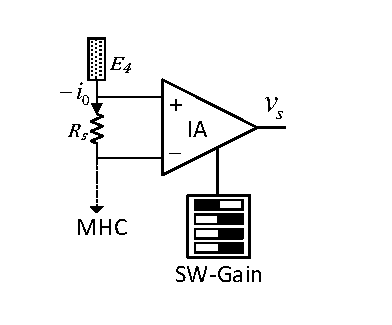
\includegraphics[width=8cm,keepaspectratio]{figure4}
	\caption{Voltage sensing circuit schematic}
	\label{fig:peak}
\end{figure}


In contrast, following signal path for the extraction of AC signal, the signal is passed through a series of filters. First, a high pass filter is used removing DC components of the signal. This was achieved by the passive filter composed by $C_4$ and $R_5$. It must be noticed that $R_5$ is virtually connected to ground (GND). Creating a filter with cut frequency given by following equation:  

\begin{align}
\label{eg:fc1}
f_c = \frac{1}{2 \pi R C} = \frac{1}{2 \pi 330K\Omega 4.7\mu f}=10.26 mHz
\end{align}

Equation \ref{eg:fc1} illustrates that practically any DC component of the impedance signal is blocked by this circuits section. The following configuration of active filters are equivalent to a second-order non-inverting filter with cut frequency given by equations~\ref{eg:fc2} and~\ref{eg:fc3}. The first Op-Amp configuration is an inverting amplifier circuit \SI{10.61}{\hertz} with a gain in DC of \num{30.30}. The second Op-Amp configuration \SI{10.26}{\hertz} with an amplification factor in DC of \num{4.70}. 


\begin{align}
\label{eg:fc2}
f_c = \frac{1}{2 \pi R C} = \frac{1}{2 \pi 10M\Omega 1.5 nf}=10.61Hz
\end{align}

\begin{align}
\label{eg:fc3}
f_c = \frac{1}{2 \pi R C} = \frac{1}{2 \pi 47K\Omega 330nf}=10.26Hz
\end{align}

%********************************** %Nomenclature found  *************************************
\nomenclature[z-rc]{RC}{Resistor Capacitor}
\nomenclature[z-dds]{DDS}{Direct Digital Synthesis}
\nomenclature[z-ic]{IC}{Integral Circuit}
\nomenclature[z-spi]{SPI}{Serial Peripheral Interface Bus}
\nomenclature[z-opamp]{Op-Amp}{Operational Amplifier}
\nomenclature[z-cmmr]{CMMR}{Common Mode Rejection}
\nomenclature[z-mhc]{MHC}{Modified Howland Circuit}
\nomenclature[z-inamp]{In-Amp}{Instrumentation Amplifier}
\nomenclature[z-adc]{ADC}{Analogue to digital converter}
\nomenclature[z-spst]{SPST}{Single Pole Single Throw}
\nomenclature[z-dc]{DC}{Direct Current} 
\nomenclature[z-ac]{AC}{Analogue Current}
\nomenclature[z-gnd]{GND}{Ground Point}
\nomenclature[z-pwv]{PWV}{Pulse Wave Velocity}


